%-----------------------------------------------------------------------------------
%	PACKAGES AND OTHER DOCUMENT CONFIGURATIONS
%----------------------------------------------------------------------------------

\documentclass[11pt]{article}

\usepackage[top=2cm, bottom=3cm, left=2cm, right=2cm]{geometry}
\setlength{\parskip}{1em}
\setlength{\parindent}{4em}
\linespread{1.25}

\newcommand{\Var}{\mathrm{Var}}

\newcommand{\Cov}{\mathrm{Cov}}

\newcommand{\plim}{\rightarrow_{p}}

\usepackage{apacite}

\usepackage{amsmath, amsfonts}
\usepackage{graphicx}
\usepackage{pdfpages}
\usepackage{bm}
\usepackage{listings}
\usepackage{multirow,array}
\usepackage{enumerate}
\usepackage{bbm}
\usepackage{subfig}
\usepackage{bbm}

\usepackage[latin1]{inputenc}

\usepackage{amssymb}

\usepackage{mathrsfs}
\usepackage{float}
\usepackage{booktabs}
\usepackage{color}
\usepackage{rotating}
\usepackage{amsthm}
\usepackage{multirow,array}
\usepackage{caption}
\usepackage{url}



\DeclareMathOperator*{\argmax}{arg\,max}
\DeclareMathOperator*{\argmin}{arg\,min}

\usepackage{fancyhdr}

\pagestyle{fancy} % Turn on the style
 % Start with clearing everything in the header and footer
% Set the right side of the footer to be the page number
\fancyfoot[R]{\thepage}

% Expectation symbol
\newcommand{\E}{\mathrm{E}}
\newcommand{\V}{\mathrm{V}}
\newcommand{\N}{\mathcal{N}}
\newcommand{\R}{\mathbb{R}} 

%----------------------------------------------------------------------------------
%	TITLE AND AUTHOR(S)
%----------------------------------------------------------------------------------

\title{Asymmetric Learning Model of Resume Building With Wage Rigidity and Costly Firings} % The article title

\author{Nathan Mather} % The article author(s) 

\date{\today} % An optional date to appear under the author(s)

\renewcommand{\contentsname}{Table of Contents}
%----------------------------------------------------------------------------------
\begin{document}
	
	
	%------------------------------------------------------------------------------
	%	TABLE OF CONTENTS
	%------------------------------------------------------------------------------
	\maketitle % Print the title/author/date block
	
	\setcounter{tocdepth}{3} % Set the depth of the table of contents to show sections and subsections only
	\tableofcontents % Print the table of contents
	
	\newpage
	%------------------------------------------------------------------------------
	% Introduction 
	%------------------------------------------------------------------------------

	\section{Introduction}
	
	Labor market models seek to strike a balance between including realistic aspects of the labor market while remaining parsimonious and understandable. Asymmetric learning models incorporate the realistic assumption that current employers will know more about their own employees than competing firms.  Acemoglu and Picshke lay out an extensive model of asymmetric information and show how it can explain employers paying for general training \cite{AP_1998} \cite{AP_1999}. While this work showed how a the reasonable assumption of assymetric information could explain the puzzle of employers paying for training, their work did not actually confirm empirically that asymmetric information is prevalent in labor markets. Uta Sch�nberg developed a strategy for empirically estimating to what extent this asymmetry exists in the market \cite{Sch_2007}. Surprisingly, Sch�nberg finds little evidence of asymmetric information in the labor market; however, the logic and anecdotal evidence supporting this assumption seems strong enough to warrant additional investigation. \par 
	
	Rather than working to empirically measure the level of asymmetric information again, I build out a model of asymmetric information with additional realistic assumptions about labor markets. The goal is to create a more realistic model and identify what implications these additional factors have for wages in various markets. The main idea and focus of my model is to investigate how wages are impacted by asymmetric information in an environment where outside firms only observe a resume like signal and are subject to sticky wages and various fixed firing costs. The model has a lot in common with the two period Acemoglu and Picshke model of asymmetric learning and general training, but is simplified in certain ways in order to focus on new assumptions and aspects of the Labor market \cite{AP_1998}.  \par
	
	Some of the key way my model differs is that employers in my model will only observe a noisy signal of worker ability. A firm that receives a good signal will consider that worker to have a high \textit{expected} ability rather than simply knowing they have high ability. I believe this departure will have more significant implications in a 3 period or more model. The second difference from the Acemoglu and Picshke model is that I assume outside firms can observe an employees resume. That is,  they can tell after period one if a worker was fired or separated from their firm, or if the firm decided to keep them. This has implications for the two period model, and will allow for a more realistic framework for labor force signals in 3 or more periods. Finally, I consider the impact of sticky wages and costly firings.  \par 
	
	The results of the model so far suggest that in an otherwise frictionless market, asymmetric information of this type will tend to lower wages and increase wage dispersion with tenure. A market with asymmetric information and sticky wages, but with high fixed costs to firing, will see relatively constant and even wages over tenure. \par
	
	In section 2.1 We start by laying out the basic structure of the model. In section 2.2 we find the equilibrium outcome in a market with no fixed costs to firing and completely flexible wages. While the initial model without wage rigidity or firing costs closely matches a simplified version of the  Acemoglu and Picshke mode, explicitly laying out the implications of the model in this setting makes the impact of wage rigidity and firing costs more clear \cite{AP_1998} \cite{AP_1999}. In section 2.3, we then consider what happens to this model if we introduce wage rigidity, but have no firing costs. Finally, in section 2.4, we consider what happens as for various firing costs. In section 3 we simulate results for various parameters to better understand the implications of the model. In section 4 we consider what the model is missing and where to expand it in the future. 
	
%----------------------------------------------------------------------------------
% Two period Model Basics 
%----------------------------------------------------------------------------------


	\section{ The Model}

	
	\subsection{Environment}
	

	The model lasts for two periods. In the first period no firm has information about any individual workers. While it is a bit of a stretch to think that firms have zero information about a potential worker, consider two new entrants to the workforce with similar skills and resumes. Firms have very little ability to gain information to distinguish between the two. While interviews could potentially help, there is some evidence that they may actually lead to less informed decision making \cite{interview_2013}. This model abstracts away from observable differences in things like education to consider the wages of workers who are similar on paper. \par

	While firms have no information about individual workers, firms do have knowledge about the workforce as a whole. Firm know workers have ability $\theta \in [0,1]$ which is  distributed over $f(\theta)$. Workers produce $\theta$ per period and supply labor inelastically. They take the highest wage offer they receive, and in the event of a tie stay with their current employer or pick randomly if unemployed.\par
	
	After working for one period a fraction $\delta$ of workers exogenously separate from their firm. Employers cannot distinguish between someone who was fired or exogenously separated. This implies firms offer a single wage to all unemployed workers in period 2 since, to employers, they all have the same resume and are identical \footnote{that is they have one year experience and are currently unemployed}. Employers can offer a different wage to workers who have not been fired or separated. These workers are distinguishable from the unemployed \footnote{they have a year of experience and are currently employed on their resume} and likely have different average characteristics. \par
	
	For the workers that do not separate, their current employers receive a noisy signal about their ability. Workers with ability $\theta$ send a good signal with probability $\theta$ and a bad signal with probability $1-\theta$. This exact specification is not crucial, we just need that higher ability implies a higher probability of sending a good signal. After receiving this signal employers choose if they want to fire employees for a fixed cost $F_C$. Employers then offer wages to their employees for period 2 conditional on this signal. After Employers offer wages to their own employees, firms can then offer wages to outside workers conditional on employment history. Workers decide where to work and produce for one more period before retiring. There are many competitive firms, so this implies a zero profit condition on all firms. The variables I will be using are summarized in table 1 below. The time line is also laid out more concisely below.\par 
 
	\begin{center}
		\textbf{{\Large Table 1}  }
	\end{center}
	\begin{center}
		\resizebox{.75\linewidth}{!}{\begin{tabular}{||c | c||} 
				\hline
				Variable & Meaning  \\ [0.5ex] 
				\hline\hline
				$\theta$ & Ability \\ 
				\hline 
				$g$ & Good Signal\\ 
				\hline
				$b$ & Bad Signal \\
				\hline
				$e$ & Employed Signal\\
				\hline
				$f$ & Fired Signal\\
				\hline
				$F_C$ &  Fixed Cost to Firing \\ 
				\hline
				$\delta$ & Exogenous separation rate \\ 
				\hline
				$w_1$ &  Period 1 Wage \\ 
				\hline
				$w_g$ & Wage After Good Signal \\
				\hline
				$w_b$ & Wage After Bad Signal \\
				\hline
				$w_e$ & Wage Offered to Worker With a Year of Employment\\
				\hline
				$w_u$ & Wage for unemployed worker\\	\hline
				$\pi$ & Profits\\[1ex] 
				\hline
			\end{tabular}
		}
	\end{center}
	
\begin{center}
	\textbf{{\Large Time line}  }
\end{center}
	\begin{enumerate}
	\setlength{\itemsep}{1mm}
	\item period 1 wage offers
	\item Workers produce output
	\item Workers Exogenously separate
	\item Workers send signal of ability 
	\item Employers decide who to fire
	\item Employers offer current employees period 2 wages conditional on signal. That is $w_g$, and $w_b$
	\item Outside Firms offer wages conditional on resume. That is $w_e$, and $w_u$
	\item Workers take the best offer and work for one more period 
	\item Workers retire 
\end{enumerate}





%----------------------------------------------------------------------------------
% Flexible Wage Model
%----------------------------------------------------------------------------------


\subsection{Flexible Wage Model}
First, we consider a model with totally flexible wages. In this model there is no reason to ever fire workers. Employers can simply lower wages to whatever level is profitable or induce a worker to quit.  We denote the expected output of employees who sent a good or bad signal in period 2 as $\E[\theta|g]$ and $\E[\theta|b]$ respectively. Proposition 1 lays out what period 2 wages will be in this model.

\textbf{Proposition 1:} Second period wages in the flexible model will be $w_g = \E[\theta|g]$,  $w_b = \E[\theta|b]$, and  $ w_u =  \frac{ \delta \E[\theta] + (1-\delta)p(b)( \E[\theta | b])}{\delta + (1-\delta)p(b)}$. All Workers who send a bad signal will quit and switch firms. 

To determine wages, we use backward induction and begin in the second period. To start, let's remain agnostic about who will quit after the first period. Let $Q$ denote the fraction of workers that do not separate and then quit. We know the wage offer to an unemployed worker for a given $Q$ is 

$$ w_u(Q) = (\delta \E[\theta] + Q \E[\theta | \text{worker quit}])/(\delta + Q)$$

We also know that employers will not pay their low signal employees more than $\E[\theta | b]$ since this would result in a loss. They also cannot pay them less since an outside employer would pay at least $\E[\theta | b]$ for any worker. This implies 

$$ w_b = \E[\theta | b] $$

Using these two equations we can show the following lemma

\textbf{Lemma 1:}  $w_u \geq w_b$

The lowest possible $w_u$ is if the pool of workers has the lowest average skill. That is, if all bad signal employees quit and no good signal employees quit. This gives us

$$\E[\theta|b] < \min w_u(Q) = \frac{ \delta \E[\theta] + (1-\delta)p(b)( \E[\theta | b])}{\delta + (1-\delta)p(b)} $$

Lemma 1 implies that all bad signal employees will quit to receive $w_u$ rather than $w_b$. If all bad signal employees quit, then any worker who is still employed after period 1 must be high skill. Thus, outside firms can infer an employed worker's ability perfectly and so 

$$ w_e = \E[\theta|g]$$

Since this is the outside offer for employed workers, current employers must match this wage to retain workers. Thus 
$$ w_g = w_e$$
Quitting would mean workers enter a pool with some low signal employees and take a wage cut to $ w_u < w_g$. So, high signal employees do not quit. Thus we have determined all period 2 wages and confirmed proposition 1. Next, we turn to period 1 wages

\textbf{proposition 2:} First period wages in the flexible model will be $$w_1 = \E[\theta]$$

Given the wages in period 2, in order to determine period one wages all we need to do is apply the zero profit condition. The period one wage will be equal to period one output plus expected profits in period two. Only good workers are retained, and employers earn zero profits on them. Thus, first period wages are just the expected output in the first period $\E[\theta]$. 

Putting this together we get $ w_g >w_1 > w_u $. That is, over time wages increase on average for good workers and decrease on average for bad workers. This increases the spread of wages over time. Additionally, we get from this model that any workers who are sending bad signals to their employers will just quit rather than face wage cuts. These conclusions match some intuition about the labor market. For example, we should expect good workers to receive higher wages on average as employers learn about their ability. Other aspects, however, seem unrealistic.  Large real wage cuts do not typically happen. Moreover, if an employer is dissatisfied with an employee, they are likely to fire them, not cut their wage and induce them to quit. In fact, in the above model no one is ever fired. If firms can costlessly lower wages the existence of any firings do not make sense. To correct this, I first introduce sticky wages. \par 

 
 %----------------------------------------------------------------------------------
 % sticky wages, no firing costs 
 %----------------------------------------------------------------------------------
 
 
\subsection{ sticky wages with no firing costs }

In this section we introduce downward wage rigidity or "stick wages" into the model. By ``downward wage rigidity" I explicitly mean that firms cannot cut wages in period 2 from what they were in period 1. We will also start by assuming that the fixed cost to firing employees, $F_C$, is zero. 

\textbf{proposition 3:} Wages in an equilibrium with no firing costs and sticky wages are  $w_1 = \E[\theta]$,  $w_g = \E[\theta|g]$,  $w_b = \E[\theta|b]$, and  $ w_u =  \frac{ \delta \E[\theta] + (1-\delta)p(b)( \E[\theta | b])}{\delta + (1-\delta)p(b)}$. The same as without sticky wages.


To solve this problem, we will again want to use backward induction. However, we now need to know which wages in the second period are stuck, i.e. equal to $w_1$. For this, it seems, we need to know $w_1$ first, creating a dilemma for backward induction. This could be solved by simply checking each possibility for an equilibrium, but we can instead determine which wages are stuck using the zero-profit condition. 

\textbf{Lemma 2:} $w_1 \in \Big(\E[\theta|b], \E[\theta|g] \Big)$


We know lemma 2 holds because We know that the profit maximizing wage offers, without wage rigidity, for firms in period 2 will be the wages offered in the flexible model. So, if the firm offers period one wages $w_1 \leq \E[\theta | b]$ they can offer the same wages as in the flexible model in period two and receive positive profits. This does not satisfy the zero-profit condition and so will not be an equilibrium. If a firm offers first period wages $w_1 \geq \E[\theta|g]$ they will not be able to lower wages in the second period. They will be paying wages higher than the maximum output and so clearly earn negative profits. Thus, this is also not an equilibrium. \par 

Lemma 2 implies $w_b = w_1$ because $w_b$ will be ``stuck". So, since firing is costless, firms will fire low signal employees. Since only high signal employees are left employed, we get the same outcome as in the flexible wage scenario. Except now bad signal employees are fired rather than quitting. 

 
 %----------------------------------------------------------------------------------
 % sticky wages and firing costs 
 %----------------------------------------------------------------------------------
 
 \subsection{sticky wages and firing costs }
 
 	 
 The sticky wage result at least acknowledges the existence of firing, but it may not be completely satisfactory either. Employers likely do not fire employees as soon as their expected output drops just below their wage. Firing employees and creating turnover can be difficult and costly for firms.  Some firms may face extremely high fixed costs to firing through legal risk, difficulty building a case for firing workers, difficulty getting managers to fire employees, or strong unions. This gives firms an incentive to hang on to some employees even if their marginal productivity is less than their wage. We incorporate this logic into the model by introducing a fixed cost to firing employees \par 
 
	%----------------------------------------------------------------------------------
	% low firing costs 
	%----------------------------------------------------------------------------------
 
	 \subsubsection{Low firing costs}
	 
	 First we consider the case of very low firing costs. This situation could apply to markets like low wage retail jobs without unions. There are likely some fixed administrative costs to firing employees, but the large risks of legal repercussions are likely much smaller than in other markets. If the fixed cost is very low, it will not alter the employer's behavior in period two compared to the model above with zero firing costs. Later we determine how low exactly this needs to be,  but for now simply consider a ``small enough" fixed cost. Firms will simply pay the fixed cost and fire their bad signal employees. While this does not alter period 2 decisions, it does alter the period one wage offer. This is because now when a firm hires an employee, they will have difficulty getting rid of them if they are bad. Wages are sticky so the worker cannot be induced to quit, and if the firm wants to fire the worker they need to pay a fixed cost. Together, this implies the marginal benefit of a newly hired worker has decreased due to this fixed cost. So, the wage offer in period one is lower. Specifically, we get
	 
	 $$ w_1 = \E[\theta] - (1- \delta)p(b)F_C$$
	 Firms may have difficulty getting rid of bad employees, but will employees ever quit on their own? If so, this would lead to a different outcome than the one outlined above. Bad employees will not ever quit on their own because their stuck wage $w_1$ will always be greater than or equal to the unemployed wage $w_u$. I prove that this is true for all fixed costs that lead to this equilibrium in the section on mixed equilibrium. Next, we determine for which fixed costs this outcome holds. These wages will be a stable equilibrium whenever firms cannot deviate and receive positive profits. If a firm deviates and keeps their bad signal employees they will have to pay them $w_1$ (because of sticky wages). These workers will not leave for another firm because $w_1 \geq w_u$. Therefore, keeping bad signal employees gives 
	 
	 $$\pi_{keep} = \E[\theta] - w1 + (1-\delta) \Big(p(g)(\E[\theta|g] - w_g) + p(b)(\E[\theta|b] - w_1 )\Big) = \E[\theta] - w_1 +  (1-\delta) \Big( p(b)(\E[\theta|b] - w_1) \Big) $$
	 
	 compared to firing them and receiving 
	 $$\pi_{fire} = \E[\theta] - w1 + (1-\delta) \Big( p(g)(\E[\theta|g] - w_g) - p(b)F_C \Big) $$
	 
	 Thus firing workers is optimal for all firms as long as the fixed cost to firing is less than the loss from holding onto a bad signal worker.
	 
	 $$ w_1 - \E[\theta|b] > F_C$$
	 
	 $$ \implies  \E[\theta] + (1- \delta)p(b)F_C -  \E[\theta|b] > F_C $$
	 
	 $$ \implies f_C < \frac{\E[\theta] -  \E[\theta|b]}{1 + p(b)(1-\delta)} $$
	 
	 
	 
	 This equilibrium implies $w_u < w_1 < \E[\theta] < w_g$. The intuition here is that in period two firms either make 0 expected profits on good signal workers or have to pay to fire bad signal workers. Given this, workers in the first period are paid below their expected first period output. While this leads to the odd conclusion that firms would be happy if their entire labor force left in the second period, this is an artifact of only having two signals for simplicity. With two signals, Employers are taking losses on firing bad employees and then just breaking even on good employees. If they had middle signal employees, they would retain some inside information about their workforce even after firing all bad worker. In this case they would not want their good employees to quit.\footnote{This discussion of results under more signals should be taken with the caveat that I have not completely solved the model for this case, and am relying only on intuition and some preliminary efforts}
	 
	 %----------------------------------------------------------------------------------
	 % Wage rigidity with High firing Costs 
	 %----------------------------------------------------------------------------------
		 
	 \subsubsection{High firing Costs  }
	 
	While in many cases the fixed costs to firing may be small, as as we outlines above above, in other markets the costs may be extremely high. For example, markets with extremely strong unions may make it very costly to fire a worker. Even in the absence of unions, strong worker solidarity or reputation effects may mean the firm incurs costs through lower productivity of current workers or lower quality future applicants. Another possibility is that a firm may be under strict legal rules about firing workers. It may be that firing workers risks paying out large legal fees. If the fixed costs become sufficiently large, it is clear that firms will not fire any employees. We will determine how large is "sufficiently large", but for now simply consider an extreme case.\par
	
	Given that no employees are fired, we now need to determine what equilibrium wages will be when firms retain both high and low signal workers. It is also clear from the above work that $w_b = w_1$ since those wages are stuck. This also implies $w_b \leq w_g$. 
	
	When considering what to offer a worker who is currently employed at a different firm, $w_e$, all a firm knows is the general distribution of worker types. So they can infer $\E[\theta|e]$ (the expected type of a worker given they are employed. We can start by noting that firms will always offer $w_e \leq \E[\theta|e]$. This is because if firms offer $w_e$ such that $ w_b < w_g \leq \E[\theta | e] < w_e$ outside firms get all workers but at an expected loss. \par 
	
	Next, consider the case where $\E[\theta|b] \geq w_b < w_e < w_g$. In this case outside firms only attract bad signal employees for a negative expected profit so this cannot be an equilibrium. Finally if $ w_e \leq w_b \leq w_g \leq \E[\theta | e]$ the outside offer attracts no workers and so outside firms earn zero profits. This has the potential to be an equilibrium. Whether or not firms have an incentive to deviate depends both on $w_g$ and assumptions about the structure of the market. 
	
	Acemoglu and Picshke assume that current employers can always move second and get the last offer in. This leads to a "winners curse" that would keep outside offers low even if $w_g < \E[\theta|e]$ \cite{AP_1998}.  Under these assumptions, the outcome $ w_e \leq w_b = w_g = w_1$ is stable.  I, however, work on the assumption that employers must set their wages first then outside firms make their offers. While the former way matches the framework of, for example, the academic market, where countering outside offers is popular, my logic more closely matches many typical labor settings. Employers have wages set and cannot validate outside offers. If an employee gets a better offer elsewhere employers often simply let the employee go. Under these assumptions if $ w_g = w_1$ than outside employers would offer $w_e = w_1 + \epsilon < \E[\theta|e]$ for a positive profit on all workers. Under my assumptions,a stable outcome is $w_b = w_1$, and $w_g = \E[\theta|e]$. With these wage offers any offer an outside firm makes will result in a loss and so they simply offer a wage low enough to attract no workers, $w_e = \E[\theta | b]$. \par 
	
	This gives us 
	
	$$ w_g = E[\theta | e] =\E[\theta]$$
	
	They will pay their bad signal employees as little as possible 
	$$ w_b = w_1$$ 
	
	unemployed workers get their expected output 
	$$ w_u = E[\theta] $$
	
	this gives a first period wage through the zero profit condition 
	$$w_1 = \E[\theta] + (1-\delta)(p(g)(\E[\theta|g] - \E[\theta]) + p(b)(\E[\theta|b] - w_1))$$
	
	
	using the fact that $p(g)\E[\theta|g] + p(b)\E[\theta|b] = \E[\theta]$ we get 
	
	$$ w_1 = \E[\theta] +  (1-\delta)(\E[\theta] - p(g)\E[\theta] - p(b)w_1)$$
	
	using the fact that $ \E[\theta] - p(g)\E[\theta] = p(b)\E[\theta]$
	
	$$ \implies  w_1 = \E[\theta] +  (1-\delta)p(b)(\E[\theta] - w_1) $$
	$$ \implies w_1 +(1-\delta)p(b)w_1 = \E[\theta] + (1-\delta)p(b)\E[\theta]$$
	
	$$ \implies w_1 = \E[\theta]$$
	
	So all workers get paid $\E[\theta]$ no one is fired and also no workers are induced to quit since quitting gets them the same wage. Firms have inside information, but they are too restricted to do anything with it. They can not lower their bad employee's wages or fire them. \par 
	
	This equilibrium will be stable whenever it is more costly to fire an employee then to keep them at this wage \footnote{ 	While I find this story fairly conniving, there is some aspect of firm behavior that still doesn't seem quite right to me. Specifically, wages are treated exogenously in the stability condition. In a later section we explore the possibility of an extension to the model that allows wage offers specific to each firm that would make wages endogenous to firm's decisions about firing employees. This extension would clear up much of the logic above and make the model more accurate, albeit much more complicated.}. That is when 
	
	$$ F_C >  w_1 - \E[\theta|b] = \E[\theta] - \E[\theta|b]$$
	
	The implication of this is that sticky wages make it impossible for firms to capitalize on their inside information in period 2 by cutting worker's wages while the high firing costs are making it impossible to use inside information for strategic firing. Thus, they earn no profits in period two and incur no costs; So, period one wages are not bid up past expected revenue in period 1. This fits the intuition that if unions are strong and firing workers is hard, wages will not disperse over time and will not increase due to employers learning about innate ability \footnote{They would likely increase do to forces outside the model, however, like human capital development. The point is that employer learning will not contribute to wage growth.}. 
	

		 
	 
	 %----------------------------------------------------------------------------------
	 % Mixed Equilibrium
	 %----------------------------------------------------------------------------------
	 
	\subsubsection{Mixed Equilibrium}
	
	
	We have outlined the two extreme cases, very low and very high fixed costs. Now consider the case between the two. That is, whenever 
	
	$$ F_C \in \left[  \frac{\E[\theta] - \E[\theta|b]}{1 + p(b)(1-\delta)} , \E[\theta] - \E[\theta|b] \right] $$
	
	In this case employers will fire a fraction of their bad signal workers $\delta_F$ until they are indifferent between firing and keeping them 
	$$  F_C = w_1 - E[\theta|b]$$ 
	
	Good signal employees need to be paid the expected output of an average worker employed in period 2, for the same reason outlined in the section above. This gives us
	
	$$ w_g(\delta_F) = \frac{p(g)\E[\theta|g] + p(b)(1-\delta_F) \E[\theta|b] }{p(g) + p(b)(1-\delta_F)} $$
	
	bad signal employees are paid the lowest wage possible $ w_b = w_1$ and unemployed get their expected output 
	
	$$ w_u = \frac{ \delta\E[\theta] + (1-\delta) p(b) \delta_F \E[\theta | b]}{  \delta + (1-\delta) p(b)\delta_F} $$
	
	by the zero profit condition we get the first period wages 
	
	$$w_1 = \E[\theta] + (1-\delta)  \bigg( p(g) \Big(\E[\theta|g] - w_g(\delta_F)  \Big) - p(b)F_C  \bigg) $$
	
	
	Given an exogenous separation rate, we can also calculate the fraction of workers fired $\delta_f$.  We have two equations for $w_1$ with the only unknown being $\delta_F$. I have solved for it below, but it not very intuitive. We can see that as the fixed cost rises the fraction of workers fall. It can also be used to solve numeric examples.
	\newcommand{\TAMEG}{\frac{\E[\theta] -  (1+(1-\delta)p(b))F_C - \E[\theta|b]}{(1-\delta)p(g)}}
	
	$$ \delta_F = \frac{p(g) \left[\TAMEG \right]}{ p(b) \left[ \E[\theta | b] - \TAMEG - \E[\theta|g] \right] } $$
	
	Returning to the question from the low firing cost section, will bad signal workers ever just quit on their own? That is, will we ever have $w_1 \geq w_u$? I show in the appendix 1 that this will never occur in a mixed equilibrium or when all bad signal workers are fired. That is as long as $F_C \leq \E[\theta] - \E[\theta|b]$.  Thus, the equilibria I outline above are stable.  \par 
	

%----------------------------------------------------------------------------------
% Numerical examples 
%----------------------------------------------------------------------------------

\section{Numerical Examples}


While the above work characterizes the equilibrium for any set of parameters, in order to visualize the impact that fixed costs and separation rates have on wages we graph a numerical example. Theta is distributed uniformly from 0 to 1 \footnote{This is discretized over 100 points in order to calulate it all in R}. We then plot the wages for each group for 200 fixed costs evenly distributed between 0 and 0.25. We stop at 0.25 because after this all wages are 0.5 and no one is fired. We do this for separation rates $\delta$ of .2, .4, .6, and .8. The results are in figure 1. \par 

First we Period 1 wages decline immediately with fixed costs as employers pay the fixed costs to fire bad employees. Eventually, however, employers stop firing all their bad signal employees and thus are paying lower fixed costs and earning profits on high signal workers which raises period one wages until they return to 0.5 where no one is fired. \par 

Next we see that wages for unemployed workers start low with a low fixed costs, since the pool of workers is filled with bad signal workers who are fired. After fixed costs reach the point where not all bad signal workers are fired, unemployed wages move up until no one is fired. A higher exogenous separation rate means higher unemployed wages because there are more average workers to dilute the pool of bad fired workers. This effect no longer matters, however, if no one is fired. \par 

Bad signal workers who are  fired simply track unemployed wages until bad signal workers are no longer fired. Bad signal workers who are not fired just track period 1 wages since their wages are stuck. \par 

Finally, good signal wages start out high. Since bad signal workers are fired and so being employed is a signal of high ability. However, as firms start retaining some of their bad signal employees they are able to underpay their good signal employees and take advantage of their inside information. 

It is interesting that the impact of exogenous separation on wages varies depending on the fixed costs. This makes sense given the model, but was not obvious to me ex-ante. This could potentially be one area to explore checking the validity of the model against empirical trends.   

\begin{figure}[H]
	\centering
	\LARGE{\textbf{Figure 1}}
	
	\subfloat{
		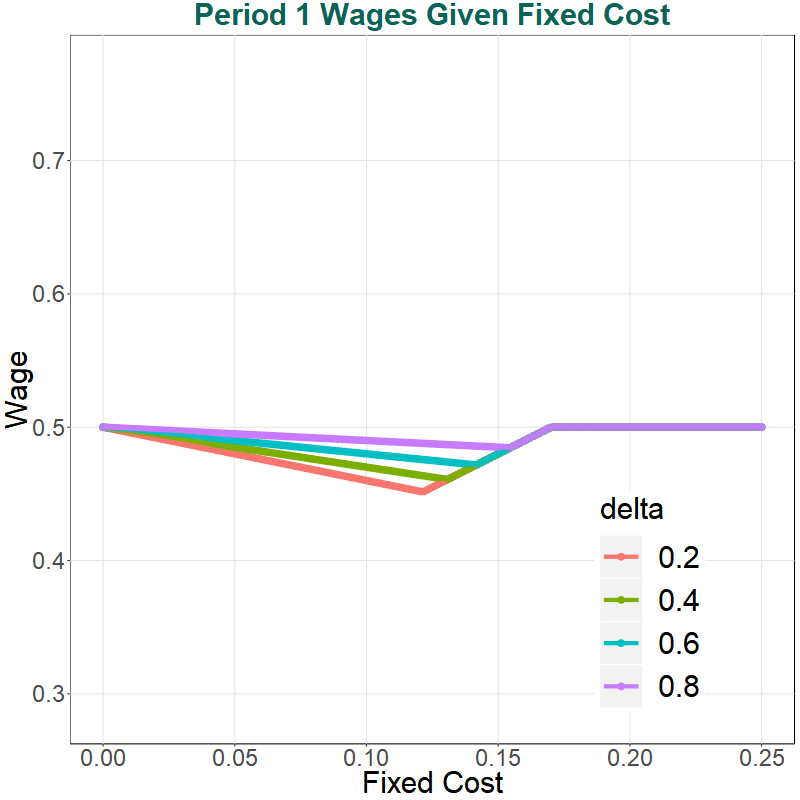
\includegraphics[width=.45\linewidth]{Period_1_Wages_Given_Fixed_Cost.png}
	}
	\subfloat{		
		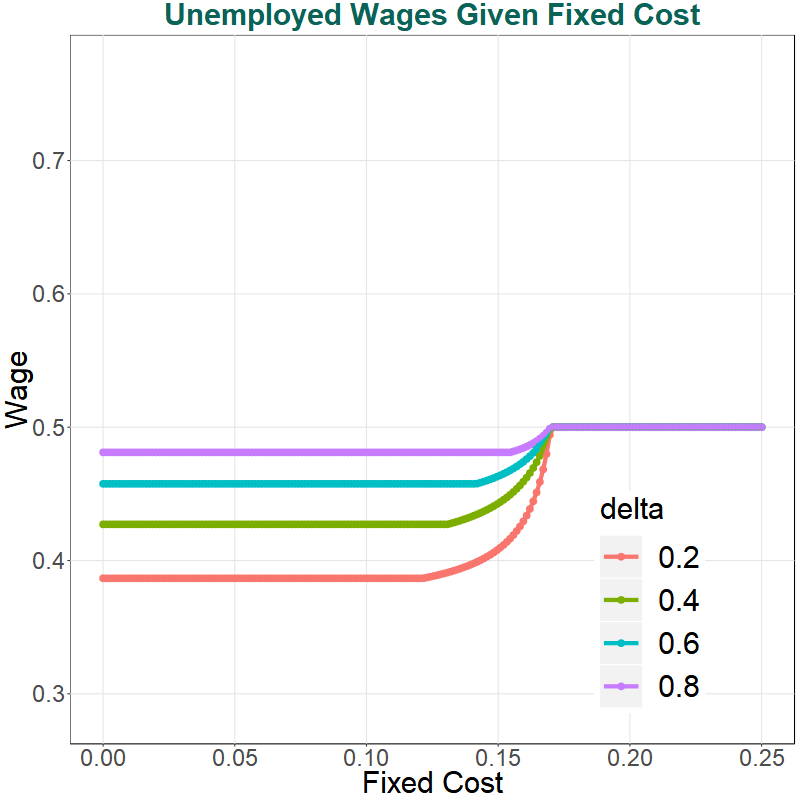
\includegraphics[width=.45\linewidth]{Unemployed_Wages_Given_Fixed_Cost.png}
	}
	\newline
	\subfloat{
	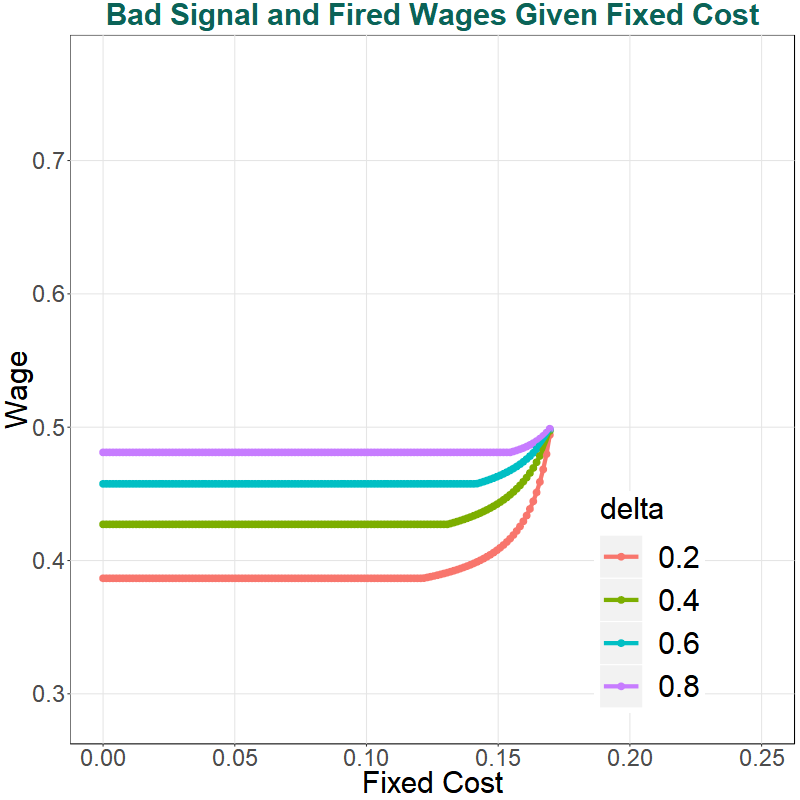
\includegraphics[width=.45\linewidth]{Bad_signal_and_fired_Wages_Given_Fixed_Cost.png}
	}
	\subfloat{
		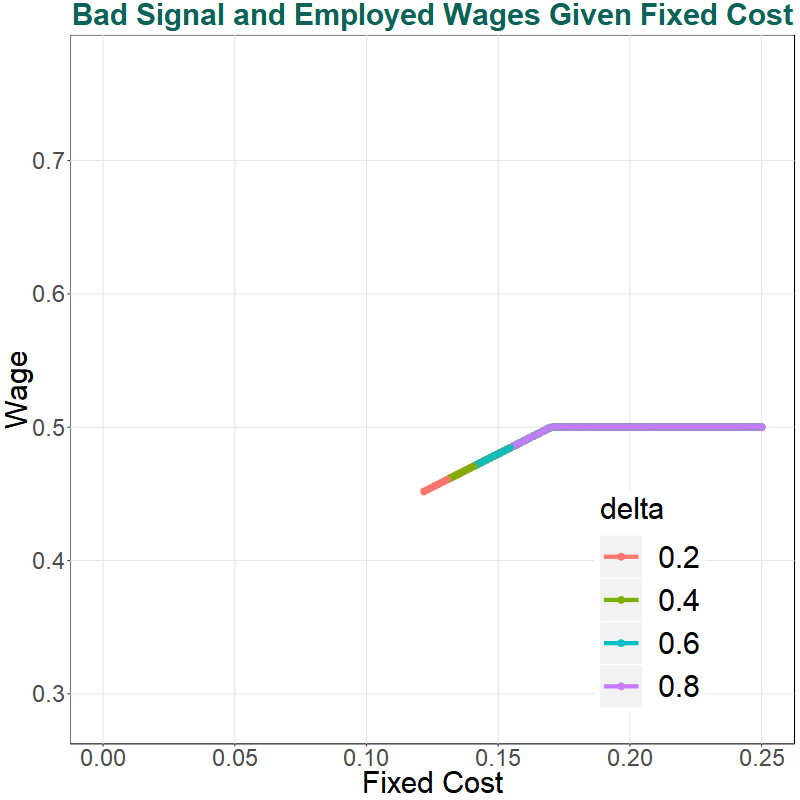
\includegraphics[width=.45\linewidth]{Bad_signal_and_employed_Wages_Given_Fixed_Cost.png}
	}
\newline
	\subfloat{
	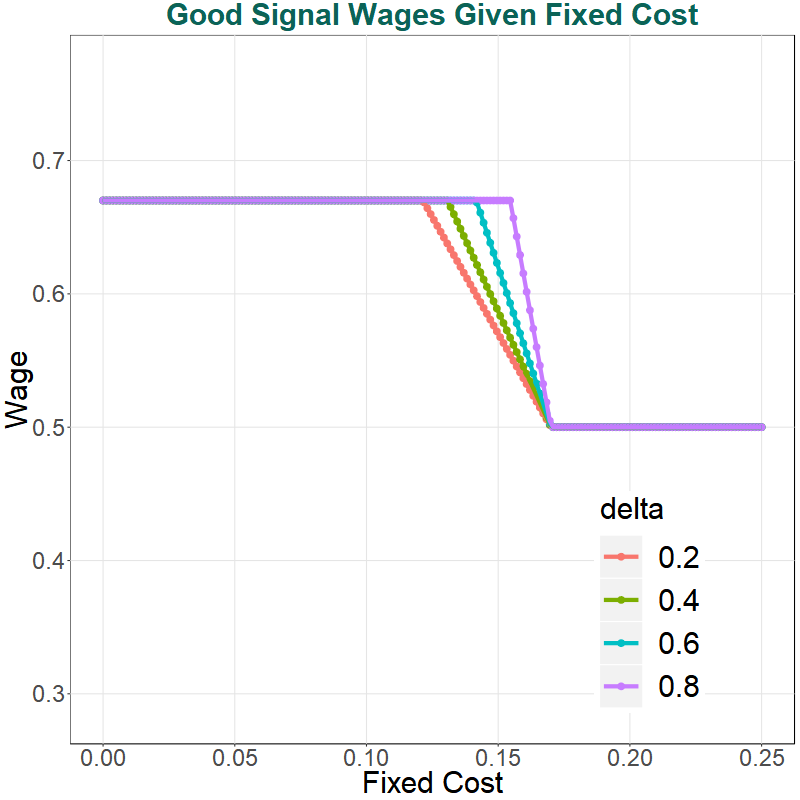
\includegraphics[width=.45\linewidth]{Good_Signal_Wages_Given_Fixed_Cost.png}
	}

	
\end{figure}

%----------------------------------------------------------------------------------
% Future Work
%----------------------------------------------------------------------------------

\section{Future work}

While I have learned a lot from working on this project, there are still many aspects of this model to consider more closely and expand upon. There are some fairly clear ways I have begun to explore for expanding the model. Adding more periods would allow us to consider more carefully how employer learning leads to changes over time. However, in my initial efforts at solving a three period model I had to rely on specific parameterizations and find a solution numerically. The initial solutions I was obtaining were also suggesting significant differences as the market jumped between various equilibria. This exploration led me to realize that perhaps a more fruitful area to expand the model first is by allowing more than two signals of ability. Perhaps even a continuous signal of ability. The Initial work on this has led me to expect the solution is also very much dependent on the distribution of ability.

 While the above considerations are a clear extension of my work, the most fundamental  area to take a closer looks is at my implicit assumption that all firms offer the same wages $w_g$ and $w_b$ after good an bad signals. This leads to a more shaky definition of a mixed equilibrium than I would like. While firms don't have additional information about other firms workers, they do know the composition of good and bad signal workers in their own firm in period two. Right now wages are essentially determine exogenously to the individual firms decision about firing and are determined by a market wide equilibrium. I think it may actually make more sense if the firm specific wages are endogenous to this decision. This would mean that, when considering weather to fire or not, firms account for the conditions I outline above as well as any impact keeping bad workers would have on firm specific wages. This will add an additional term to the $w_1 - \E[\theta|b] > F_C$ condition that determines when firms fire employees. Something like $ w_{1j}(\delta_{Fj}) - \E[\theta|b] + \frac{\partial w_{1j}(\delta_{Fj})}{\partial \delta_{Fj}} > F_C$. Where $w_{1j}$ is the firm specific wage and $\delta_{Fj}$ is the firm specific fraction of bad employees fired. While this seems manageable and comparable to what I have already done, the new term is dependent on the size of the firm, their distribution of workers, and period 1 wages. While I have not had time to fully work out the math on this realization, my initial investigation is suggesting that this adds significant complexity to the problem. That being said, I think the story makes more sense in this setting and if I continue the project I will start here. \par 
 
 Aside from mechanical extensions to the model, the set up would make investigating discrimination fairly straightforward. We could introduce two groups. Discrimination would show up by considering if employers misread good signals as bad signals with some probability for minority groups. We could also add in training to see if the conclusions of Acemoglu and Picshke hold up with these additional assumptions. 




\section{Conclusion}
Overall, the model makes generally unsurprising predictions about wages in an asymmetric information setting with sticky wages and fixed costs to firing. That being said, incorporating sticky wages and fixed costs into a model of asymmetric information and confirming the intuition for how we expect these assumptions to interact is a useful exercise. Some interesting predictions are the trend in period one wages as fixed costs rise and the heterogeneous impact of exogenous separation given various fixed costs. While it may be difficult to bring this model convincingly to data in it's current form, there are multiple promising areas of extension to allow this framework to better fit the labor markets that we see in practice. 



%------------------------------------------------------------------------------
% Appendix 1 
%------------------------------------------------------------------------------

\section{Appendix}


\ Proof of $w_1 \geq w_u$ when $F_C \leq \E[\theta] - \E[\theta|b]$ :

	
	In order to prove that in mixed equilibrium and equilibrium where all bad workers are fired that no bad workers voluntarily quit, We need to show that $ w_1 \geq w_u$  when $F_C \leq \E[\theta] - \E[\theta|b]$. To do this I first derive an alternative expression for $w_1$ using the fact that in a mixed equilibrium $F_C = w_1 - \E[\theta|b]$. plugging this into the original equation for $w_1$ under a mixed equilibrium we get  
	
	$$ w_1 = \E[\theta] + (1 - \delta) \Big[ p(g) \Big( \E[\theta|g] - w_g(\delta_F) \Big) - p(b) \Big(w_1 - \E[\theta|b] \Big) \Big]
	$$

If we solve for $w_1$ this simplifies to 
$$
w_1' = \frac{  \E[\theta] + (1 - \delta) \Big[ p(g) \Big( \E[\theta|g] - w_g(\delta_F) \Big) + p(b)\E[\theta|b] \Big] }{ 1 + (1 - \delta)p(b) }
$$

Note that this is exactly true for the mixed equilibrium and it is lower than the period one wage if $F_C < w_1 - \E[\theta|b]$ (i.e. in the equilibrium where all bad workers are fired). Thus if we show  $ w_1' \geq w_u$ we will have proved this for all $ F_C \leq w_1 - \E[\theta|b]$, i.e. the Equilibrium where everyone is fired and all mixed equilibrium. So we need to show 

$$
\frac{  \E[\theta] + (1 - \delta) \Big[ p(g) \Big( \E[\theta|g] - w_g(\delta_F) \Big) + p(b)\E[\theta|b] \Big] }{ 1 + (1 - \delta)p(b) } \geq \frac{ \delta\E[\theta] + (1-\delta) p(b) \delta_F \E[\theta | b]}{  \delta + (1-\delta) p(b)\delta_F} 
$$

rearranging terms and canceling like terms gives 
$$
p(b)\delta_f\E[\theta] + (\delta + (1-\delta)p(b)\delta_F)(p(g)(\E[\theta|g] - w_g(\delta_F)) + \delta P(b) \E[\theta|b] \geq p(b)\delta_F \E[\theta|b] + \delta p(b) \E[\theta]
$$

Now moving everything to one side, combining terms, and expanding $w_g(\delta_F)$ we can get the expression 
$$
p(b) \Big(\E[\theta] - \E[\theta|b] \Big) \Big(\delta_F - \delta \Big) + \Big( \delta + (1-\delta)p(b)\delta_F \Big) p(g) \left[ \E[\theta|g] - \frac{p(g)\E[\theta|g] + p(b)(1-\delta_F)\E[\theta|b]}{p(g) + p(b)(1-\delta_F)} \right] \geq 0
$$

this term is increasing in $\delta_F$. So, it will hold in general if it holds when $\delta_F = 0$. If  $\delta_F = 0$ then we get 

$$-\delta p(b) \Big[ \E[\theta] - \E[\theta|b] \Big] + \delta p(g) \Big[ \E[\theta|g] - \E[\theta] \Big] 
$$

$$ \implies p(g)\E[\theta|g] + p(b)\E[\theta|b] - \E[\theta] \Big( p(g) + p(b) \Big) = \E[\theta] - \E[\theta] = 0 \geq 0
$$
and the inequality is still weakly satisfied.  

%------------------------------------------------------------------------------
% bib
%------------------------------------------------------------------------------


\bibliographystyle{apacite}
\bibliography{References}
	
	%------------------------------------------------
	% end doc
	%------------------------------------------------
\end{document}





